\documentclass[]{article}

% Imported Packages
%------------------------------------------------------------------------------
\usepackage{amssymb}
\usepackage{amstext}
\usepackage{amsthm}
\usepackage{amsmath}
\usepackage{enumerate}
\usepackage{fancyhdr}
\usepackage[margin=1in]{geometry}
\usepackage{graphicx}
\usepackage{extarrows}
\usepackage{setspace}
\usepackage{parskip}
\usepackage{color}
%------------------------------------------------------------------------------

% Header and Footer
%------------------------------------------------------------------------------
\pagestyle{plain}  
\renewcommand\headrulewidth{0.4pt}                                      
\renewcommand\footrulewidth{0.4pt}                                    
%------------------------------------------------------------------------------

% Title Details
%------------------------------------------------------------------------------
\title{Deliverable \#3}
\author{SE 3A04: Software Design II -- Large System Design}
\date{March 27, 2023}                                
%------------------------------------------------------------------------------

% Document
%------------------------------------------------------------------------------
\begin{document}

\maketitle	

\section{Introduction}
\label{sec:introduction}
% Begin Section

\subsection{Purpose}
\label{sub:purpose}
% Begin SubSection
The purpose of this document is to provide detailed design for the carpool app that can looked upon implementation.  The objective is to take the overview of the system and its architecture and transform it into designs that describes the app's composition and behaviour. The intended audience for this document includes software developers and engineers, systems design architects, and other potential stakeholders who may benefit from an understanding of the system design.
% End SubSection

\subsection{System Description}
\label{sub:system_description}
% Begin SubSection

The system is organized into a multiple sections, each fulfilling a requirement of the product. These include Update Account, Default Home View, Database, Dispatch Ride, Arrival Response, and User Authentication. Within these sections, controllers are used to interact with both the user and the databases, as well as other sections to support the function of the application. The controllers also determine what pages are displayed to the user and the functions of the pages, and the logic and decision-making that determines which pages are displayed are illustrated in section 2 using state diagrams. The pages represent the user interface layer of the system. The use cases of our system and the orders of interactions and responses are shown using sequence diagrams. The overarching structure of the system and its sections can be seen in the detailed class diagram in Section 4.    



% End SubSection

\subsection{Overview}
\label{sub:overview}
% Begin SubSection
The document will be organized by sections based on the type of UML diagram.

In Section 2, the behaviour for all controller classes will be visualized in the form of a state chart diagram.

In Section 3, the behaviour for all use cases will be visualized in the form of a sequence diagram.

Section 4, the entire system's structure and interaction will be visualized in the form of a detailed class diagram.

At the end of the document, there is a record which represents the division of labour of all contributors to this deliverable.

% End SubSection

% End Section

\section{State Charts for Controller Classes}
\label{sec:state_charts_for_controller_classes}
% Begin Section

\pagebreak

\begin{figure}[h]
	\centering
	\includegraphics[width=28em]{assets/d3_state_legend.png}
	\caption{Legend}
	\label{fig:acd}
\end{figure}

\pagebreak

\begin{figure}[h]
	\centering
	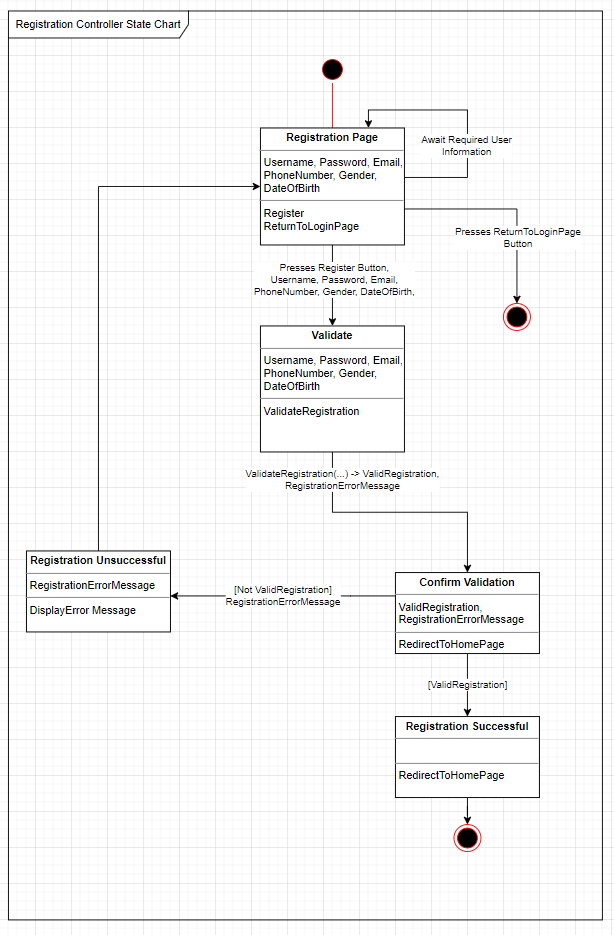
\includegraphics[width=30em]{assets/D3_2.PNG}
	\caption{Registration Controller State Diagram}
	\label{fig:acd}
\end{figure}
\pagebreak

\begin{figure}[h]
	\centering
	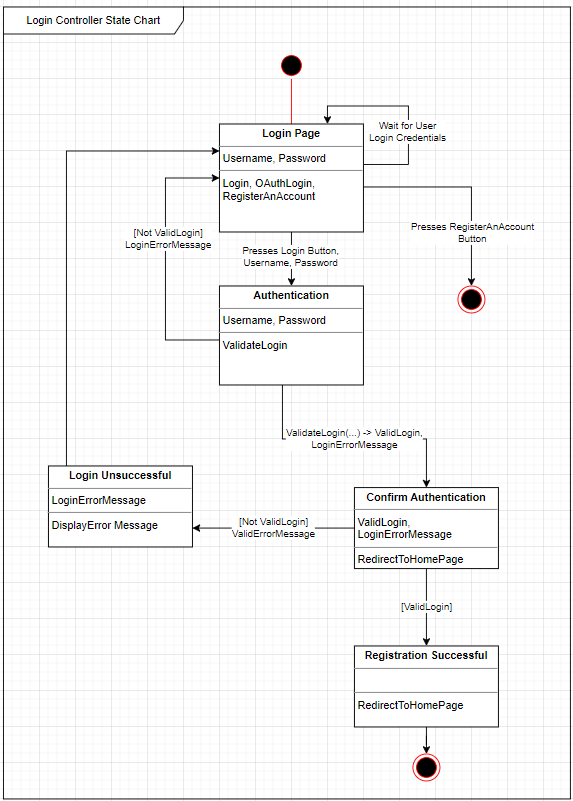
\includegraphics[width=30em]{assets/D3_3.PNG}
	\caption{Login Controller State Chart}
	\label{fig:acd}
\end{figure}
\pagebreak

\begin{figure}[h]
	\centering
	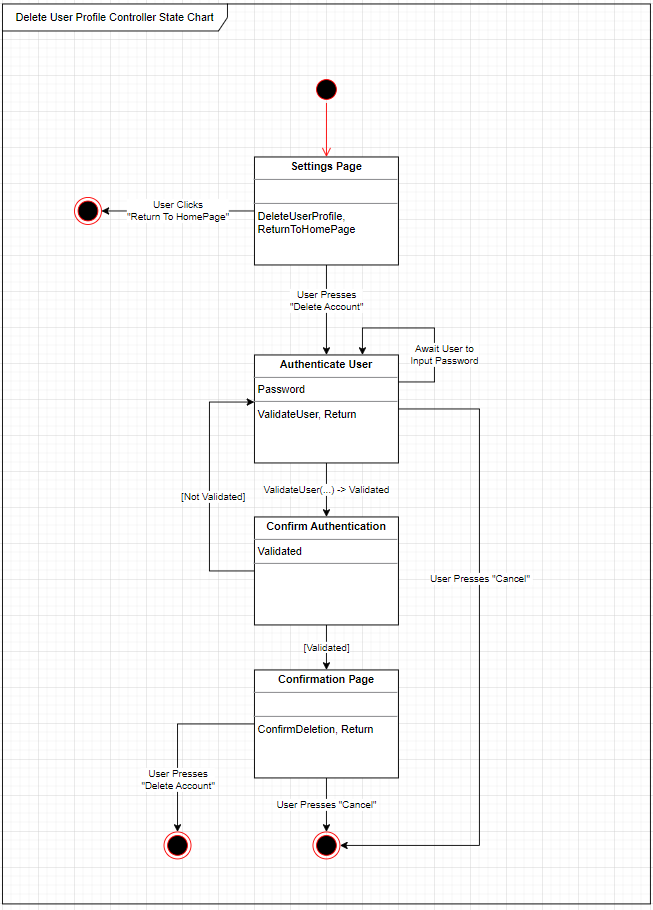
\includegraphics[width=30em]{assets/D3_4.PNG}
	\caption{Delete User Profile Controller State Diagram}
	\label{fig:acd}
\end{figure}
\pagebreak

\begin{figure}[h]
	\centering
	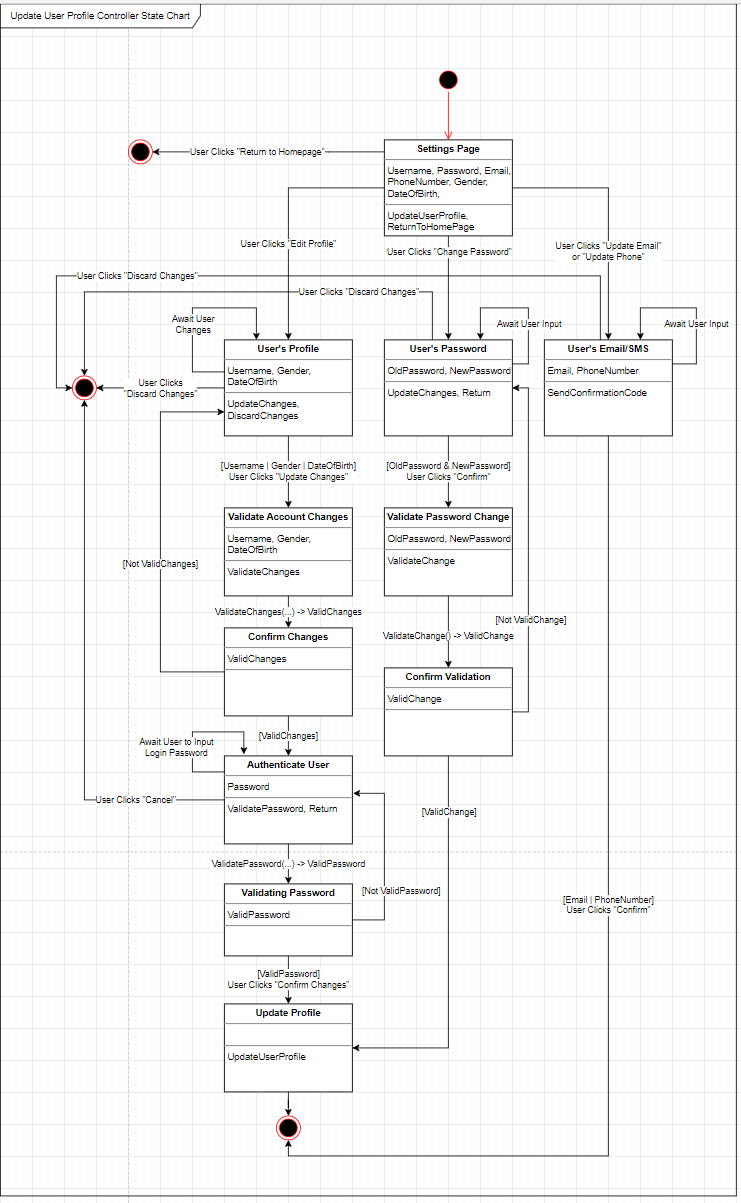
\includegraphics[width=25em]{assets/D3_5.PNG}
	\caption{Update User Profile Controller State Diagram}
	\label{fig:acd}
\end{figure}
\pagebreak

\begin{figure}[h]
	\centering
	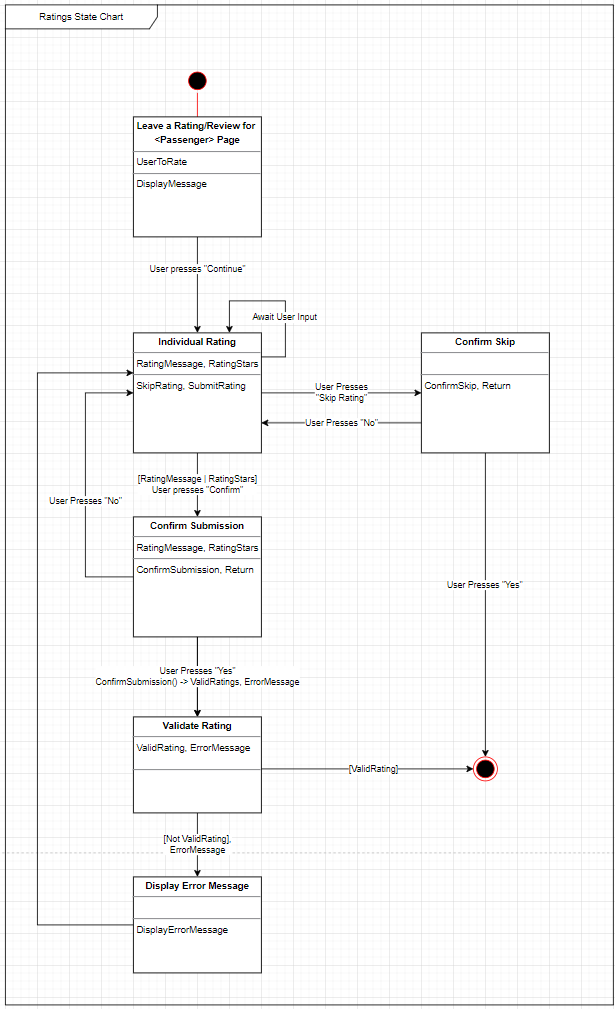
\includegraphics[width=25em]{assets/D3_6.PNG}
	\caption{Ratings Controller State Diagram}
	\label{fig:acd}
\end{figure}
\pagebreak

\begin{figure}[h]
	\centering
	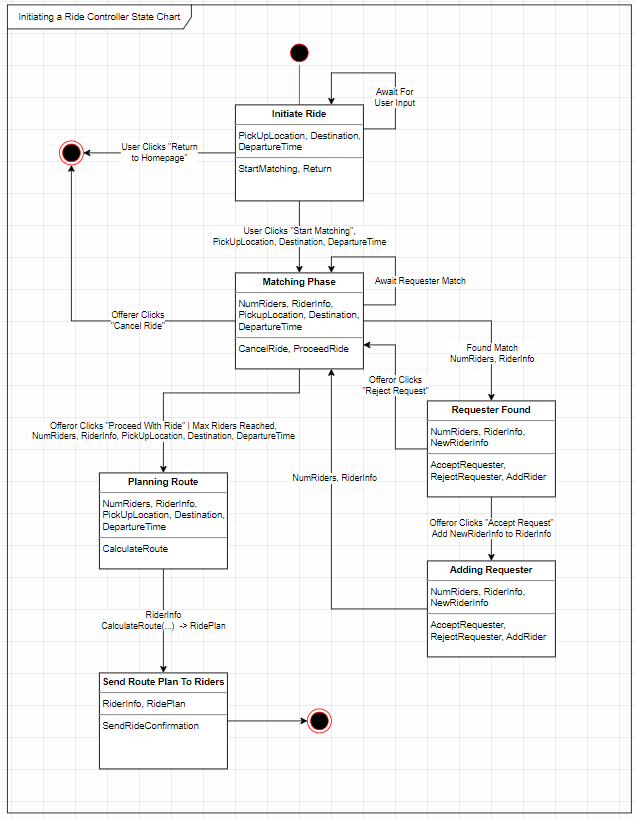
\includegraphics[width=25em]{assets/D3_7.PNG}
	\caption{Initiate Ride Controller State Diagram}
	\label{fig:acd}
\end{figure}
\pagebreak

\begin{figure}[h]
	\centering
	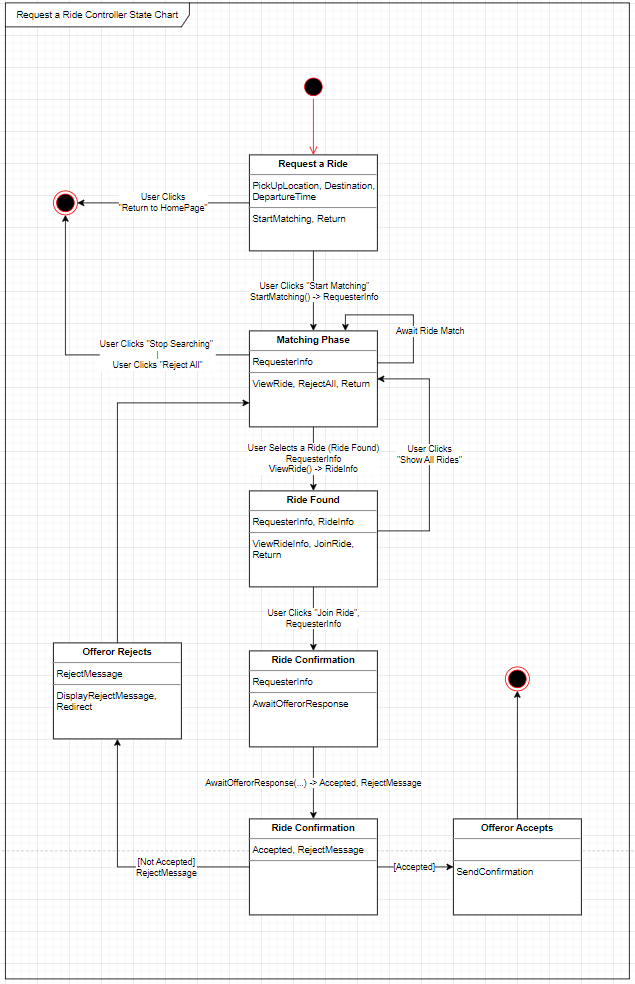
\includegraphics[width=25em]{assets/D3_8.PNG}
	\caption{Request a Ride Controller State Diagram}
	\label{fig:acd}
\end{figure}
\pagebreak

\begin{figure}[h]
	\centering
	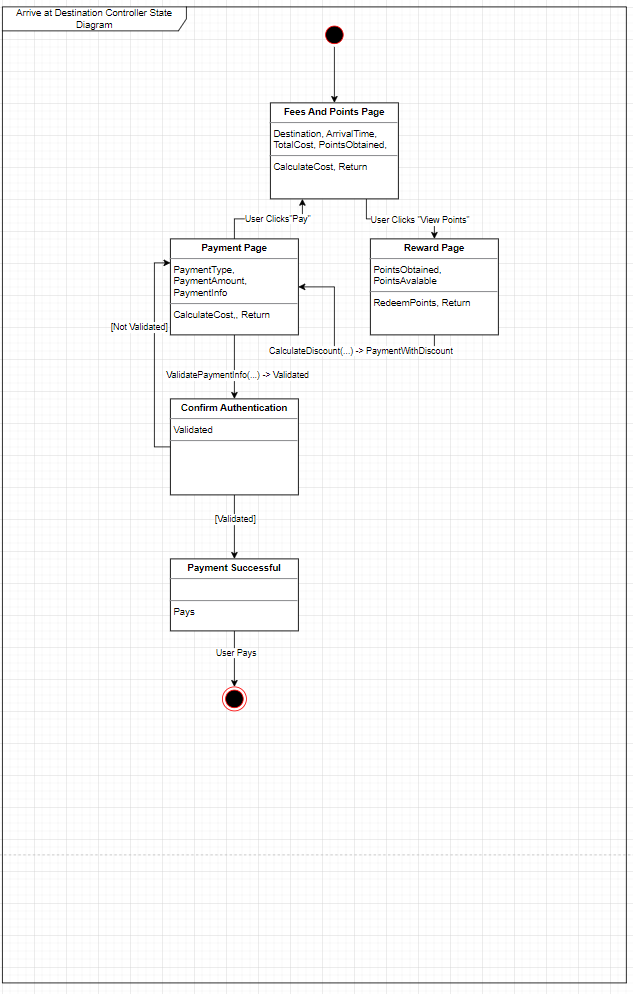
\includegraphics[width=25em]{assets/D3_9.PNG}
	\caption{Arrive at Destination Controller State Diagram}
	\label{fig:acd}
\end{figure}
\pagebreak

\begin{figure}[h]
	\centering
	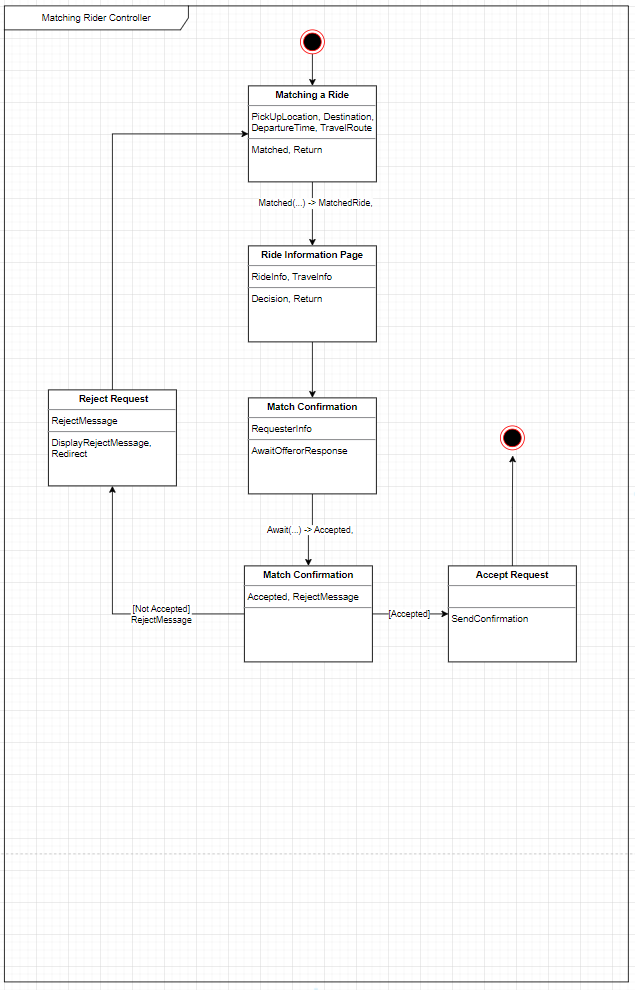
\includegraphics[width=25em]{assets/D3_10.PNG}
	\caption{Matching Rider Controller State Diagram}
	\label{fig:acd}
\end{figure}
\pagebreak

\begin{figure}[h]
	\centering
	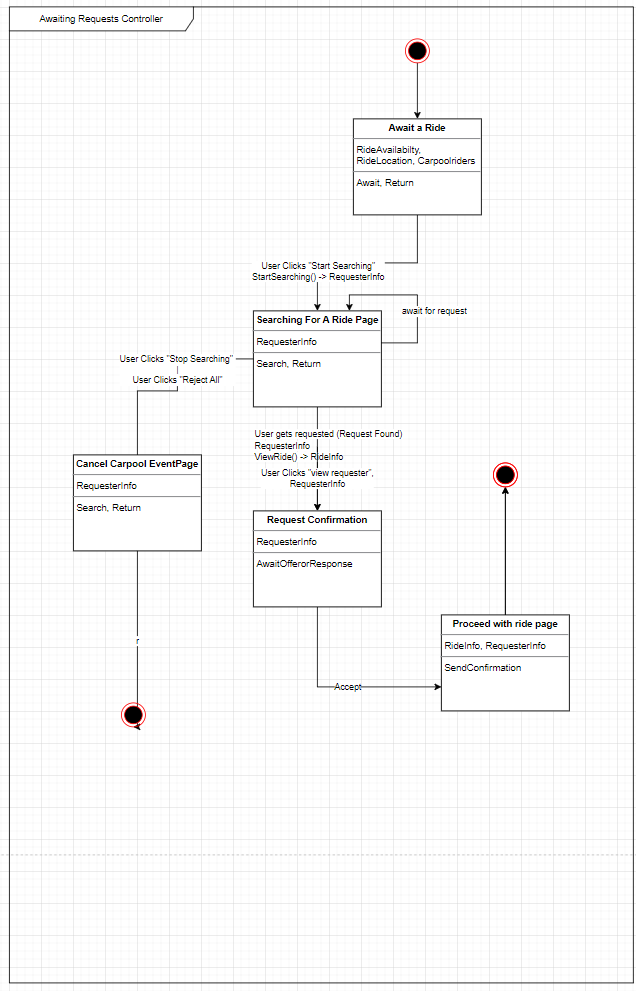
\includegraphics[width=25em]{assets/D3_11.PNG}
	\caption{Awaiting Requests Controller State Diagram}
	\label{fig:acd}
\end{figure}


% End Section

\pagebreak
\section{Sequence Diagrams}
\label{sec:sequence_diagrams}
% Begin Section

\begin{figure}[h]
	\centering
	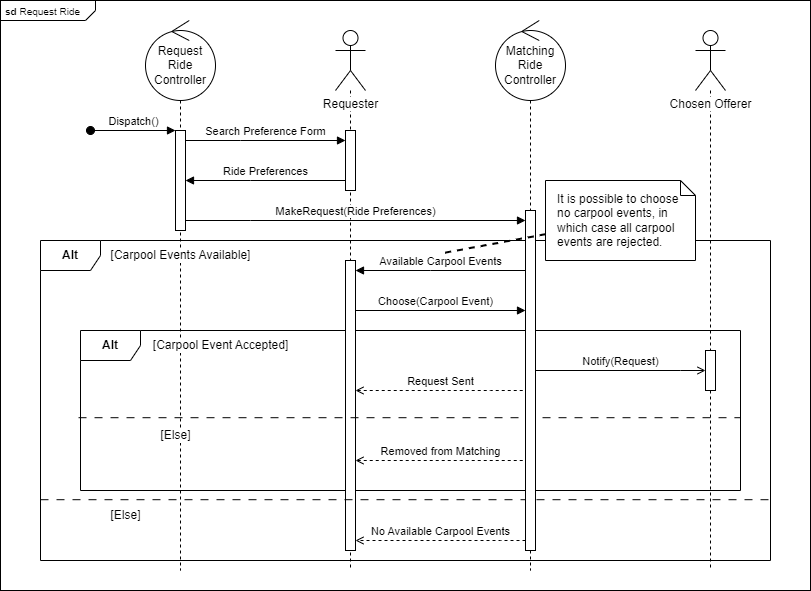
\includegraphics[width=25em]{assets/D3_12.PNG}
	\caption{Request Ride Sequence Diagram}
	\label{fig:acd}
\end{figure}

\begin{figure}[h]
	\centering
	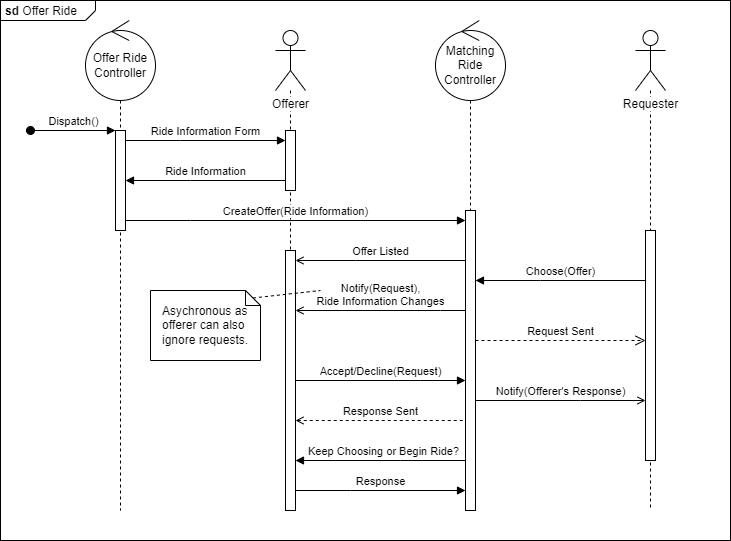
\includegraphics[width=25em]{assets/D3_13.PNG}
	\caption{Offer Ride Sequence Diagram}
	\label{fig:acd}
\end{figure}

\pagebreak
\begin{figure}[h]
	\centering
	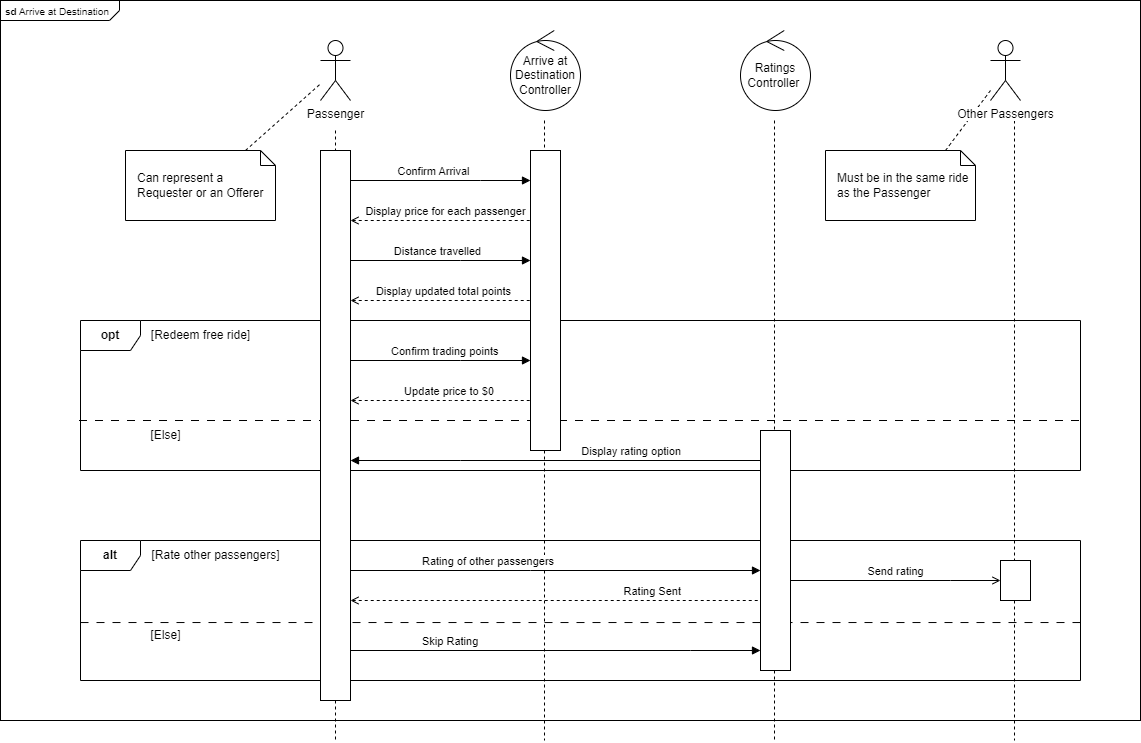
\includegraphics[width=25em]{assets/D3_16.PNG}
	\caption{Arrive at Destination Sequence Diagram}
	\label{fig:acd}
\end{figure}

\begin{figure}[h]
	\centering
	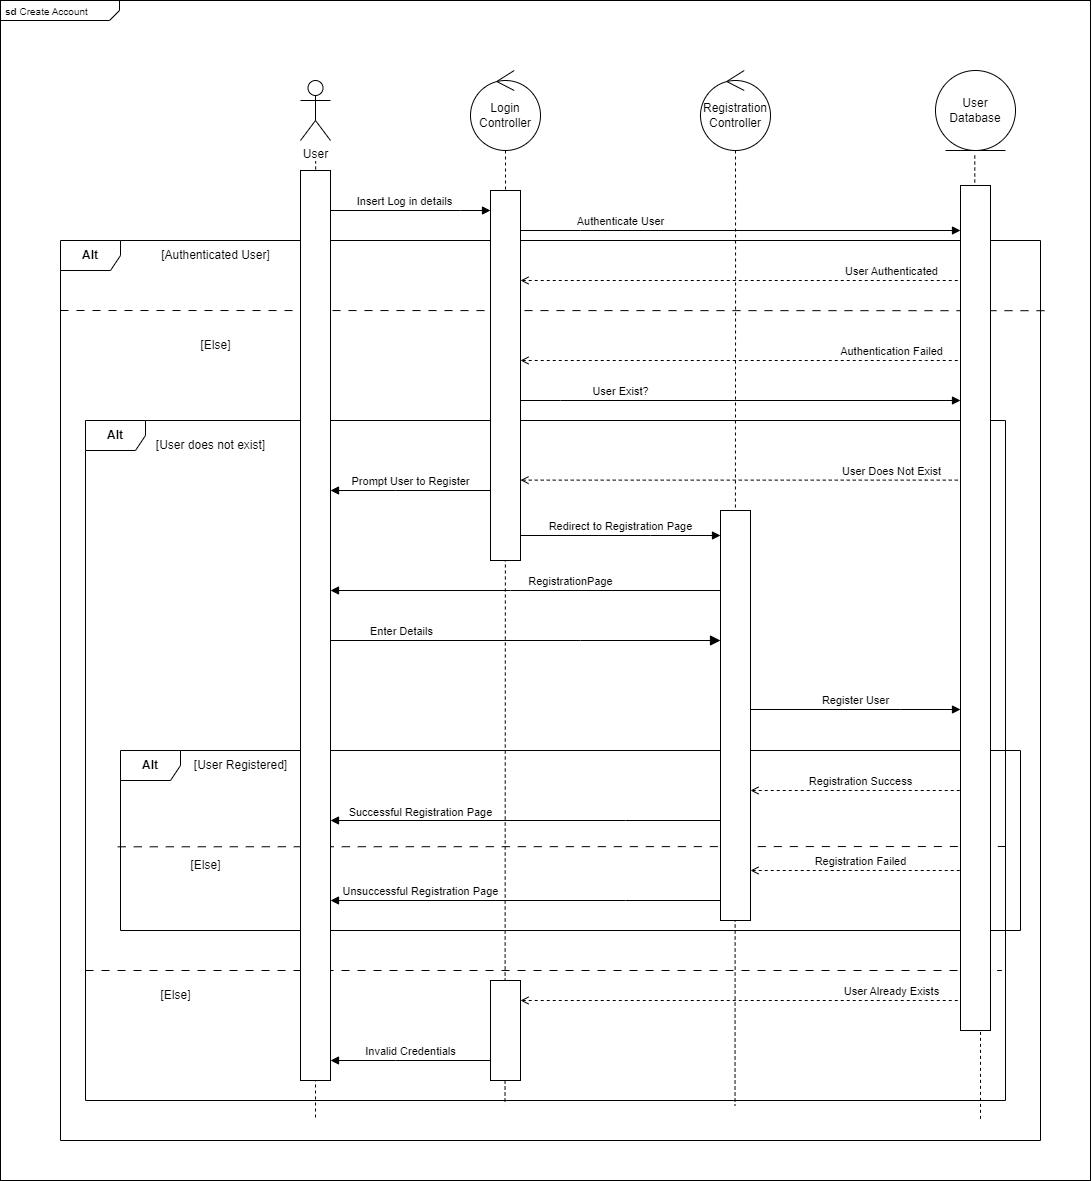
\includegraphics[width=25em]{assets/D3_15.PNG}
	\caption{Login/Create Account Sequence Diagram}
	\label{fig:acd}
\end{figure}

\pagebreak
\begin{figure}[h]
	\centering
	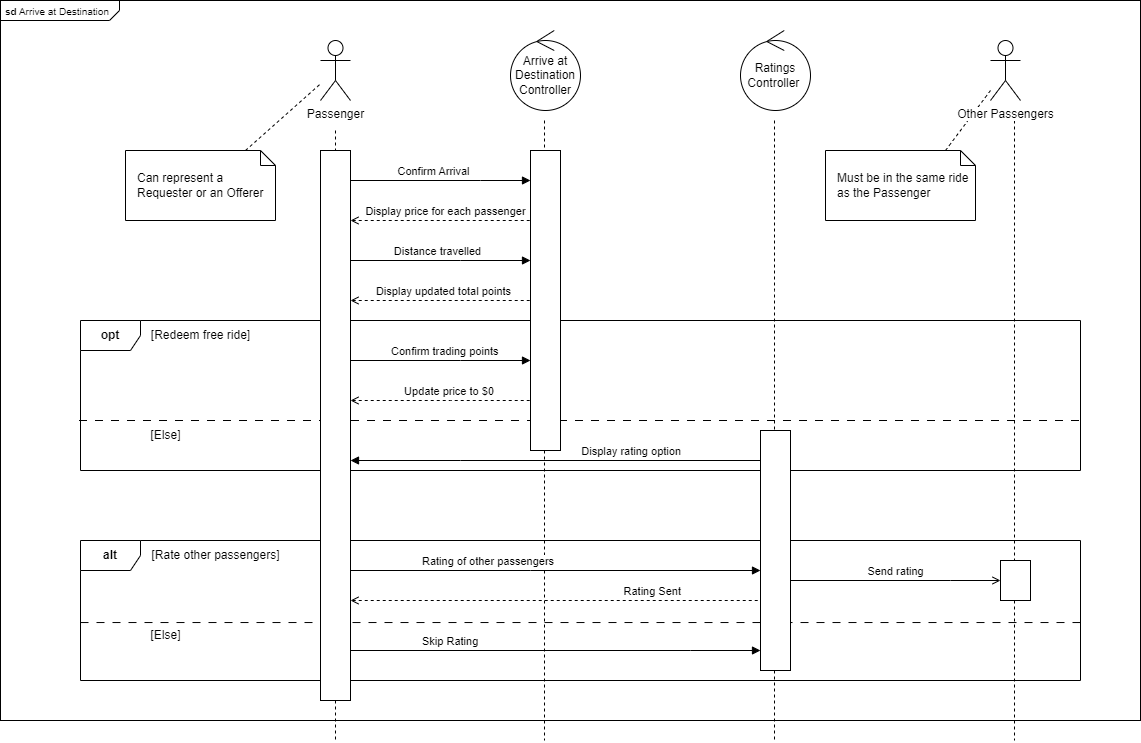
\includegraphics[width=25em]{assets/D3_16.PNG}
	\caption{Remove Account Sequence Diagram}
	\label{fig:acd}
\end{figure}

\begin{figure}[h]
	\centering
	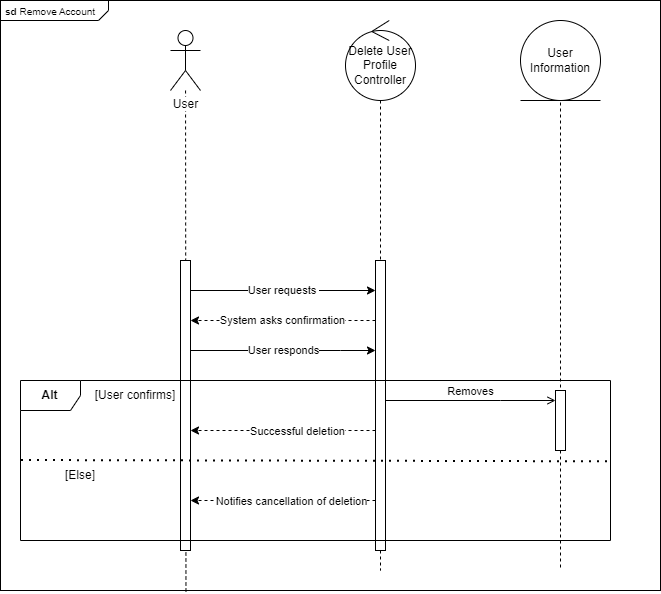
\includegraphics[width=25em]{assets/D3_17.PNG}
	\caption{Update Account Sequence Diagram}
	\label{fig:acd}
\end{figure}

% End Section

\section{Detailed Class Diagram}
\label{sec:detailed_class_diagram}
% Begin Section

\pagebreak
\begin{figure}[h]
	\centering
	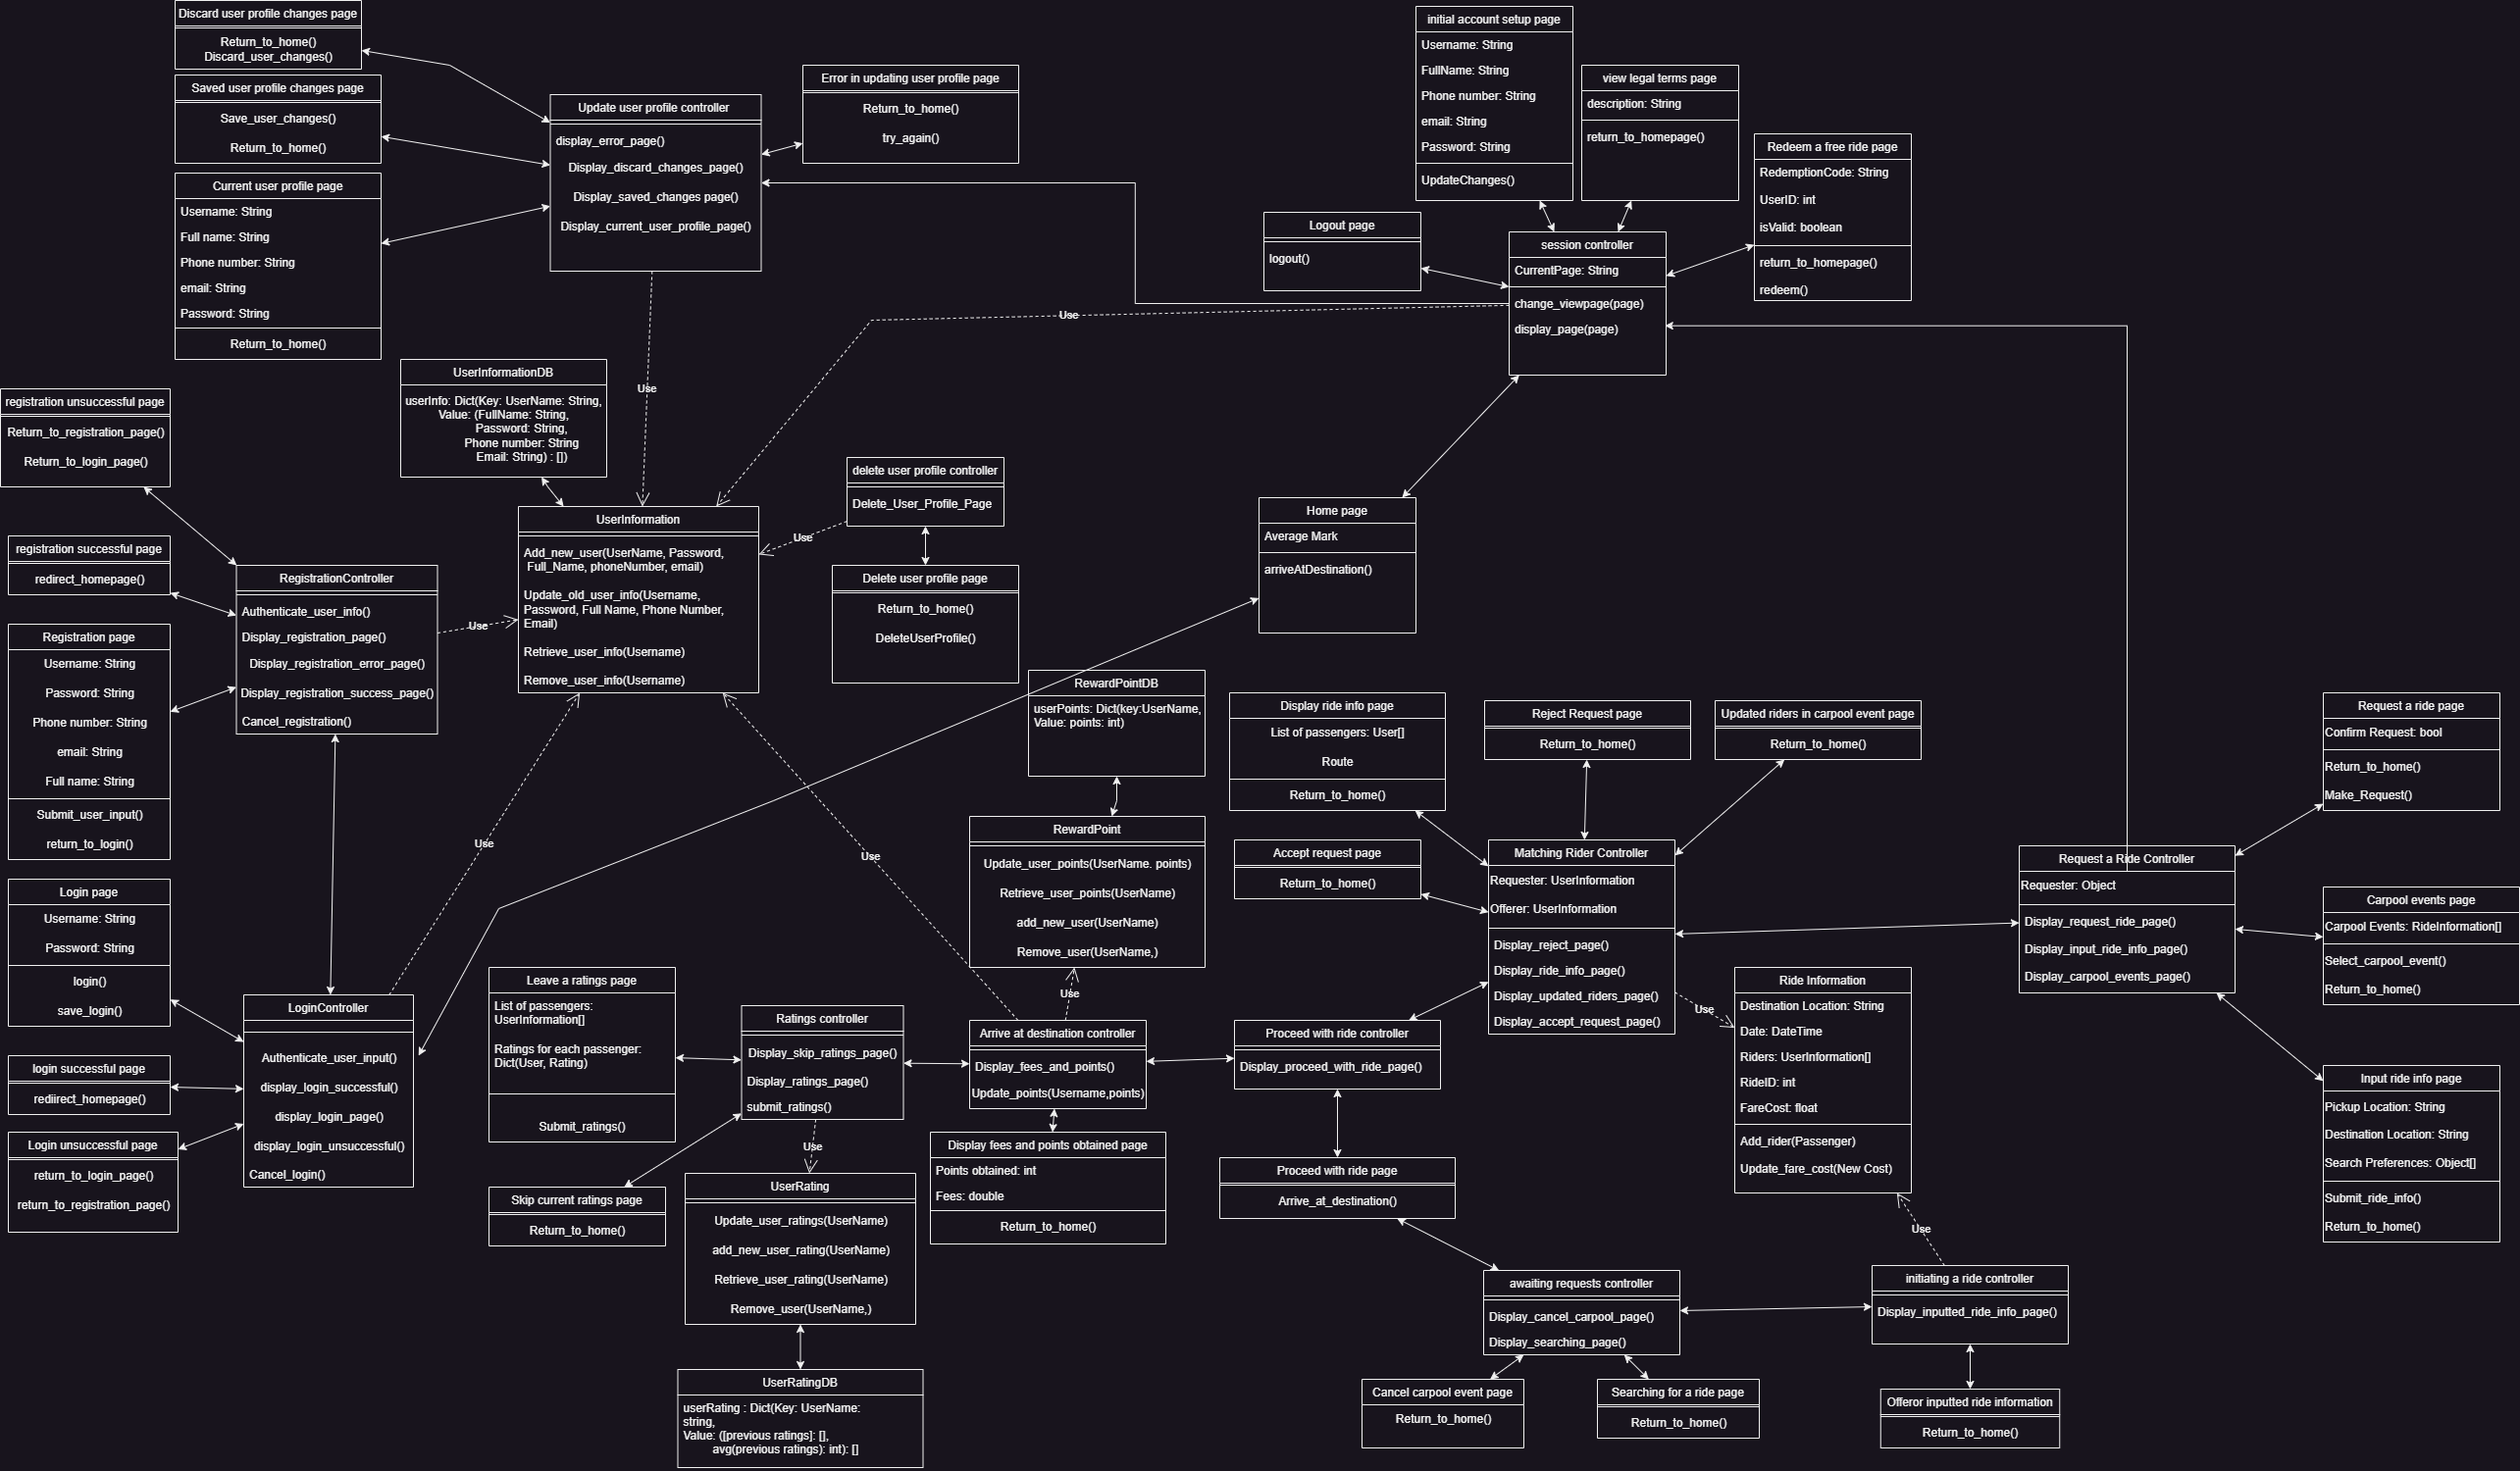
\includegraphics[width=50em]{assets/D3_classDiagram.PNG}
	\caption{Detailed Class Diagram}
	\label{fig:acd}
\end{figure}

% End Section

\appendix
\section{Division of Labour}
\label{sec:division_of_labour}
% Begin Section
Include a Division of Labour sheet which indicates the contributions of each team member. This sheet must be signed by all team members.
\begin{center} \begin{tabular} {|c|p{35em}|}
	\hline
	\textbf{Team Member} & \textbf{Contribution} \\
	\hline \hline
	Adam Mak & Purpose, Overview, Request and Offer Ride sequence diagram, contributed to the detailed class diagram.\\
	& Signed by: Adam Mak\\
	\hline
	Eric Chen & State Diagrams: Update User Profile Controller, Registration Controller, Login Controller, Delete User Profile Controller, Ratings Controller, Initiating a Ride Controller, Request a Ride Controller, Legend. Contributed to the detailed class diagram.\\
	& Signed by: Eric Chen\\
	\hline
	Justin Ho & Class diagrams layout, organization and connections. Class attributes and methods. Fixed errors from previous deliverable \\
	& Signed by: Justin Ho\\
	\hline
	Ahmad Hamadi &Await Requests Controller State, Login Controller State Chart, initiate ride Controller State Chart, Controller State Chart, Arrive at destination Controller State Chart, Matching Rider Controller State Chart, Contributed to detailed class diagram. \\
	& Signed by: Ahmad Hamadi  \\
	\hline
	Kevin Ishak & Create Account Sequence diagram,Arrive at Destination Sequence diagram and Assisted in creating some of the classes for the Detailed Class Diagram. \\
	& Signed by: Kevin Ishak \\ 
	\hline
	Jonathan Jiang & Update account sequence diagram, Remove account sequence diagram, System Description, Overview, contributed to discussions. \\
	& Signed by: Jonathan Jiang \\
	\hline
\end{tabular} \end{center}
% End Section

\newpage
\section*{IMPORTANT NOTES}
\begin{itemize}
	\item You do \underline{NOT} need to provide a text explanation of each diagram; the diagram should speak for itself
	\item Please document any non-standard notations that you may have used
	\begin{itemize}
		\item \emph{Rule of Thumb}: if you feel there is any doubt surrounding the meaning of your notations, document them
	\end{itemize}
	\item Some diagrams may be difficult to fit into one page
	\begin{itemize}
		\item It is OK if the text is small but please ensure that it is readable when printed
		\item If you need to break a diagram onto multiple pages, please adopt a system of doing so and thoroughly explain how it can be reconnected from one page to the next; if you are unsure about this, please ask me
	\end{itemize}
	\item Please submit the latest version of Deliverable 1 and Deliverable 2 with Deliverable 3
	\begin{itemize}
		\item They do not have to be a freshly printed versions; the latest marked versions are OK
	\end{itemize}
	\item If you do \underline{NOT} have a Division of Labour sheet, your deliverable will \underline{NOT} be marked
\end{itemize}


\end{document}
%------------------------------------------------------------------------------